\documentclass[12pt,fleqn]{exam}
\usepackage{pifont}
\usepackage{dingbat}
\usepackage{amsmath,amssymb}
\usepackage{epsfig}
\usepackage{upgreek}
\usepackage[super]{nth}
\usepackage[colorlinks=true,linkcolor=black,anchorcolor=black,citecolor=black,filecolor=black,menucolor=black,runcolor=black,urlcolor=black]{hyperref}
\usepackage[letterpaper, margin=0.75in]{geometry}
\addpoints
\boxedpoints
\pointsinmargin
\pointname{pts}

\usepackage[activate={true,nocompatibility},final,tracking=true,kerning=true,factor=1100,stretch=10,shrink=10]{microtype}
\usepackage[american]{babel}
\usepackage[T1]{fontenc}
\usepackage{fourier}
\usepackage{isomath}
\usepackage{upgreek,amsmath}
\usepackage{amssymb}
\usepackage{graphicx}
\usepackage{tikz}

\newcommand{\dotprod}{\, {\scriptzcriptztyle\stackrel{\bullet}{{}}}\,}

\newcommand{\reals}{\mathbf{R}}
\newcommand{\lub}{\mathrm{lub}} 
\newcommand{\glb}{\mathrm{glb}} 
\newcommand{\complex}{\mathbf{C}}
\newcommand{\dom}{\mbox{dom}}
\newcommand{\range}{\mbox{range}}
\newcommand{\cover}{{\mathcal C}}
\newcommand{\integers}{\mathbf{Z}}
\newcommand{\vi}{\, \mathbf{i}}
\newcommand{\vj}{\, \mathbf{j}}
\newcommand{\vk}{\, \mathbf{k}}
\newcommand{\bi}{\, \mathbf{i}}
\newcommand{\bj}{\, \mathbf{j}}
\newcommand{\bk}{\, \mathbf{k}}
\DeclareMathOperator{\Arg}{\mathrm{Arg}}
\DeclareMathOperator{\Ln}{\mathrm{Ln}}
\newcommand{\imag}{\, \mathrm{i}}

\usepackage{graphicx}
\usepackage{color}
\shadedsolutions
\definecolor{SolutionColor}{rgb}{0.8,0.9,1}
\newcommand\AM{\textsc{am}}
\newcommand\PM{\textsc{pm}}
     
\newcommand{\quiz}{1}
\newcommand{\term}{spring}
\newcommand{\due}{Saturday, 28 January 2023 \PM}
\newcommand{\class}{MATH 102}
\begin{document}
\large
\vspace{0.1in}
\noindent\makebox[3.0truein][l]{\textbf{\class}}
\textbf{Name:} \hrulefill \\
\noindent \makebox[3.0truein][l]{\textbf{Bonus \quiz, \term \/ \the\year}}
%\textbf{Row and Seat}:\hrulefill\\
\vspace{0.1in}

\documentclass[tikz,border=5pt]{standalone}

\begin{document}
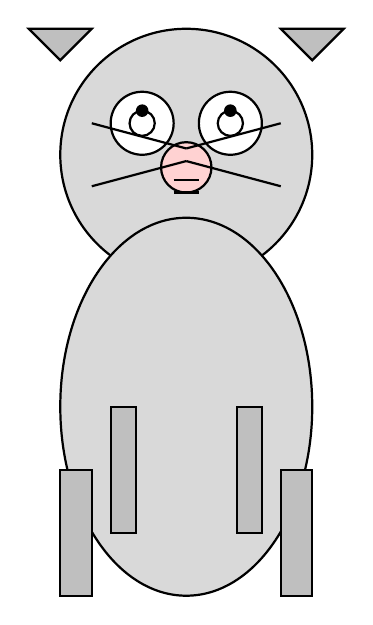
\begin{tikzpicture}[thick, scale=0.8]

% Head
\draw[fill=gray!30] (0,0) circle (2);

% Ears
\draw[fill=gray!50] (-2,1.5) -- (-2.5,2) -- (-1.5,2) -- cycle;
\draw[fill=gray!50] (2,1.5) -- (2.5,2) -- (1.5,2) -- cycle;

% Eyes
\draw[fill=white] (-0.7,0.5) circle (0.5);
\draw[fill=white] (0.7,0.5) circle (0.5);
\draw (-0.7,0.5) circle (0.2);
\draw (0.7,0.5) circle (0.2);
\fill (-0.7,0.7) circle (0.1);
\fill (0.7,0.7) circle (0.1);

% Nose and mouth
\draw[fill=pink!70] (0,-0.2) circle (0.4);
\draw (-0.2,-0.4) -- (0.2,-0.4);
\draw (-0.2,-0.6) -- (0.2,-0.6);

% Whiskers
\draw (0,0.1) -- (-1.5,0.5);
\draw (0,0.1) -- (1.5,0.5);
\draw (0,-0.1) -- (-1.5,-0.5);
\draw (0,-0.1) -- (1.5,-0.5);

% Body
\draw[fill=gray!30] (0,-4) ellipse (2 and 3);

% Legs
\draw[fill=gray!50] (-1.2,-4) rectangle (-0.8,-6);
\draw[fill=gray!50] (1.2,-4) rectangle (0.8,-6);
\draw[fill=gray!50] (-2,-5) rectangle (-1.5,-7);
\draw[fill=gray!50] (2,-5) rectangle (1.5,-7);

\end{tikzpicture}
\end{document}



To earn five bonus points,  you must do the following:
\begin{enumerate}
\item Register for our online homework.
\item Read the course syllabus.
\item Write your name in the blank above as it appears in MyBlue.

\item Answer the following questions.  Digitize your work and upload it to Canvas.
\end{enumerate}


\begin{questions} 

\question  \underline{\phantom{xxxxx}} (yes / no)  Have you registered for our online homework system?

\question \underline{\phantom{xxxxx}} (yes / no)  Have you read the course syllabus?

\question If you have a name that you prefer to your name in MyBlue, what is it?

\begin{solution}[1.0in]
\end{solution}
\question Please tell me something about yourself that might help me remember your name.

\begin{solution}[2.0in]
\end{solution}

\question Please tell me something about your best experience in learning mathematics.
\begin{solution}[2.0in]
\end{solution}

\end{questions}

\end{document}


   
\end{questions}


\end{document}

